\documentclass{standalone}

\usepackage{amssymb}
\usepackage{amsthm}
\usepackage{amsmath}


\usepackage{tikz}
\usetikzlibrary{shapes,backgrounds,calc,patterns}
\usepackage{venndiagram}


\begin{document}
    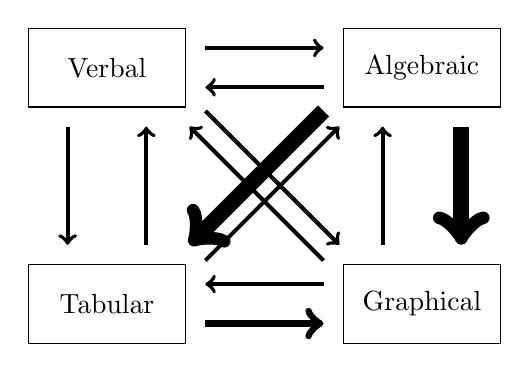
\begin{tikzpicture}
\draw (-3,2) rectangle (-1,1);
\node at (-2,1.5) {Verbal};
\draw (1,2) rectangle (3,1);
\node at (2,1.5) {Algebraic};
\draw (-3,-1) rectangle (-1,-2);
\node at (-2,-1.5) {Tabular};
\draw (1,-1) rectangle (3,-2);
\node at (2,-1.5) {Graphical};

\draw[->,line width = 2mm]  (2.5,.75) -- (2.5,-.75);  %algebraic - graphical
\draw[->,line width = .5mm]  (1.5,-.75) -- (1.5,.75); % graphical - algebraic 
\draw[->,line width = .5mm] (-2.5,.75) -- (-2.5,-.75); % verbal - tabular
\draw[->,line width = .5mm] (-1.5,-.75) -- (-1.5,.75); % tabular - verbal
\draw[->,line width = .5mm] (-.75,1.75) -- (.75,1.75); % verbal - algebraic
\draw[->,line width = .5mm] (.75,1.25)-- (-.75,1.25); % algebraic - verbal
\draw[->,line width = 1mm] (-.75,-1.75) -- (.75,-1.75); % tabular - graphical
\draw[->,line width = .5mm] (.75,-1.25)-- (-.75,-1.25); % graphical - tabular
\draw[->,line width = .5mm] (-.75,-.95) -- (.95,.75); % tabular - algebraic
\draw[->,line width = 2mm] (.75,.95) -- (-.95,-.75); % algebraic - tabular
\draw[->,line width = .5mm] (-.75,.95) -- (.95,-.75); % verbal - graphical
\draw[->,line width = .5mm] (.75,-.95) -- (-.95,.75); % graphical - verbal

\end{tikzpicture}
\end{document}